\section{Counting the remaining words}\label{q:forest-section}

We complete the trace estimate by counting the words left after
\Cref{q:many-unlit,q:rank,q:singletons}.  The arithmetic estimates have
removed words with many unlit occurrences, large constraint rank, or many
singletons.  The remaining equality patterns admit a short description
by a forest.  Its size bound will hold simultaneously for all padding
coefficients; this uniformity allows us to sum the padding weights only
after counting the patterns.

\subsection{Positive blocks and their geometry}

Retain the notation for a closed word of length $2k$ from the trace
expansion: its displacements are $D_i=\varepsilon_i hq_i d_i$, its
departure offsets are $\xi_i$, and the two halves have unequal
consecutive tuples $d_i$.  Recall that $S_1$ counts singleton column
labels and $U$ counts unlit occurrences of nonsingleton labels.  A
position is \emph{perfect} if every column occurrence at that position
is a lit nonsingleton.  All other positions are \emph{imperfect}; their
number $I$ satisfies
\begin{equation}\label{q:imperfect-count}
 I\le S_1+U.
\end{equation}
Fix a word and designation satisfying lit consistency, and a residue
configuration for which the integrand $R|\Delta G|$ in
\Cref{q:mixed-difference} is nonzero.  Since $\Delta G\ne0$, at least
one term of its defining alternating sum has $G=1$; fix such a hybrid.
All lit nonsingleton coordinates have their forced
values in every hybrid.  Also, $R>0$ supplies every padding
divisibility.  Thus every perfect step is positive in this hybrid,
and every main vertex satisfies $\sigma_j=1$.

Within each half, split every maximal interval of consecutive perfect
positions into blocks of $s=\lfloor L^{1/10}\rfloor$ positions, followed
by one shorter block if necessary.  Their number $B$ satisfies
\begin{equation}\label{q:block-count}
 B\ll 1+k/s+S_1+U,
\end{equation}
with an absolute constant.  Each block is a positive path whose
vertices all survive the prohibited-word deletion.

\begin{lemma}[Geometry of perfect blocks]\label{q:block-intervals}
In each such block, the occurrences of every column prime form an
interval of consecutive positions.  No nonempty subinterval of the
block has total displacement zero.
\end{lemma}

\begin{proof}
If the interval assertion fails, choose across all columns two
consecutive occurrence groups having the shortest gap.  Let $i$ be
the last position in the first group and $i'$ the first in the next,
and let $p$ be their common prime.  The prime $p$ is absent from
$i+1,\ldots,i'-1$.  Every label in the substring
$i,\ldots,i'-1$ has interval-shaped uses, since otherwise it would
give a shorter gap.  Positivity at the departures of steps $i$ and
$i'$ gives
\[
 p\mid \sum_{a=i}^{i'-1}D_a,
 \qquad\text{hence}\qquad
 p\mid \sum_{a=i+1}^{i'-1}D_a.
\]
The length $i'-i$ cannot be two: the latter sum would be one
displacement whose tuple and padding both omit $p$, while $p\nmid h$.
The substring therefore has length at least three.  It is a forward
prohibited word, with its suffix starting at its second step.
Pass to a minimal prohibited contiguous subword, allowing reversal.
Positivity survives these operations, and its starting vertex is
one of the main vertices.  This contradicts $\sigma_j=1$ there.

For the second assertion a single displacement is nonzero.  In any
subinterval of length at least two, the first and last tuples differ.
Indeed, if they agreed in every column, the interval assertion would
make every tuple in that subinterval equal, contrary to the
nonbacktracking condition.  Choose a first-step prime $p$ absent
from the last tuple.  If the total displacement were zero, deleting
the first step would leave a suffix sum divisible by $p$.  In a
two-step subinterval this is impossible, because $p$ does not divide
the last displacement.  In length at least three it makes the
subinterval forward prohibited.  Minimal descent gives the same
contradiction.  A reversed subword may begin at the end of the block;
this endpoint is also a main vertex.  At the end of the closed word
it is its initial vertex, so the survival condition still applies.
\end{proof}

\subsection{A forest code independent of the coefficients}

An equality pattern in a column is the partition of its $2k$ positions
according to equality of their prime labels; the numerical prime values
are not part of the pattern.  In this subsection we count the union of
these patterns over all numerical label values, padding choices, signs,
and surviving hybrids that satisfy the indicated rank and occurrence
bounds.

\begin{lemma}[Forest coding]\label{q:forest-code}
Suppose that
\[
 S_1\le L^{1/4},\qquad U\le L^{1/50},\qquad
 r=\lfloor L^{1/50}\rfloor,
\]
and that, in every column, there are no $r$ pairs
\eqref{q:rank-pair} whose $2r$ vectors are jointly independent.  Consider
lit-consistent terms of \Cref{q:mixed-difference} with a nonzero integrand.  The
equality patterns that can occur in any one column belong to a set
of cardinality at most $\exp(Ck)$, for an absolute constant $C$.
This set can be chosen independently of all numerical coefficients
and padding choices.  Consequently there are at most $\exp(CJk)$
combined column patterns.
\end{lemma}

\begin{proof}
Fix one realization and one column.  Let $\mathcal Z$ be its set of
distinct labels and let $\mathcal V$ be the real vector space with
basis $(e_z)_{z\in\mathcal Z}$.  If the label at position $a$ is
$z_a$, define its formal departure offsets by
\[
 v(i)=\sum_{a<i}t_a e_{z_a},\qquad
 t_a=D_a/p_{z_a}.
\]
The coefficients $t_a$ do not use the prime values in this column.
Choose an inclusion-maximal collection of pairs
$(e_z,v(i)-v(i'))$, where $i,i'$ are lit occurrences of $z$, whose
combined vectors are independent.  If there are $m$ pairs, their
span $D_0$ has dimension $2m<2r$.

Choose a basis of $\mathcal V/D_0$ from the images of the coordinate
vectors.  Call the corresponding labels \emph{regular} and the
other labels \emph{omitted}.  There are exactly $2m<2r$ omitted
labels.  Write $\bar v$ and $\bar e_z$ for images in the quotient.
For a regular label $z$, all lit starts lie on one affine line
parallel to $\bar e_z$.  Otherwise some difference
$v(i)-v(i')$ would be outside $D_0+\mathbb R e_z$; since
$e_z\notin D_0$, adjoining that pair would contradict maximality.
The regular directions are nonzero and jointly independent.  For each
regular label $z$ with a lit occurrence, let
\[
 \ell_z=\bar v(i)+\mathbb R\bar e_z,
 \qquad i\text{ any lit occurrence of }z.
\]
The preceding argument makes this line independent of the choice of
$i$.  The lines so defined are distinct, since their directions are
independent.

Compress each constant run in each perfect block to one run-entry.
By \Cref{q:block-intervals}, a given label occurs in at most one run
per block.  A regular run of label $z$ has quotient increment
\begin{equation}\label{q:run-increment}
 \left(\sum_{a\text{ in the run}}D_a/p_z\right)\bar e_z\ne0.
\end{equation}
The inequality uses the nonzero-subinterval assertion of
\Cref{q:block-intervals}.  Cut the runs at omitted entries and at
block boundaries.  This leaves at most $(2r+1)B$ nonempty regular
segments and at most $2rB$ omitted run-entries.  The parameter bounds
and \eqref{q:block-count} give
\begin{equation}\label{q:segment-count}
 (2r+1)B\ll L^{0.92}.
\end{equation}

Each regular run of label $z$ starts and ends on $\ell_z$, and
\eqref{q:run-increment} says that its endpoints are distinct.  A
transition from a $z$-run to a $z'$-run is therefore a common point of
$\ell_z$ and $\ell_{z'}$.  We encode these incidences by a simple
bipartite graph: one vertex represents each line used by the regular
segments, and one vertex represents each distinct projected transition
point.  Join a transition point to the two lines of its transition,
identifying vertices whenever the same line or point recurs.  Include
an isolated line vertex if it occurs only in one-run segments.
There are at most $2k$ line vertices and at most $2k$ point vertices.

This graph is a forest.  A simple cycle would pass through distinct
line vertices, and thus through distinct independent directions.
On each of its lines the two adjacent point vertices are distinct.
The displacements around the cycle would consequently give a
linear relation among the regular directions with every coefficient
nonzero, a contradiction.

A regular segment gives a walk in this forest.  It has no immediate
reversal: a walk line--point--same line would repeat an adjacent run
label, and a walk point--line--same point would contradict
\eqref{q:run-increment}.  A walk without immediate reversal in a
forest is the unique simple path between its endpoints.  Therefore
the ordered pair of line endpoints recovers all run labels of the
segment.  Equal endpoints encode a one-run segment.

Figure~\ref{fig:q-forest-incidence} illustrates this decoding.  The
graph records only incidences; the numerical positions of the points
will not enter the code.
\begin{figure}[ht]
\centering
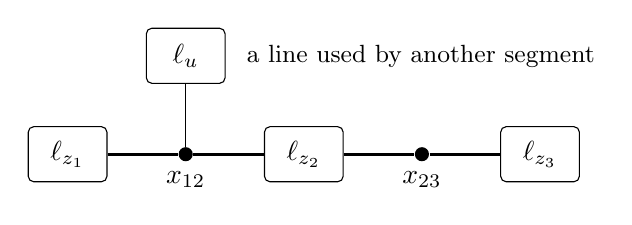
\begin{tikzpicture}[
  line vertex/.style={draw,rectangle,rounded corners=2pt,
                     minimum width=10mm,minimum height=7mm},
  point vertex/.style={circle,fill,inner sep=1.8pt}]
\node[line vertex] (l1) at (0,0) {$\ell_{z_1}$};
\node[point vertex,label=below:$x_{12}$] (p1) at (1.5,0) {};
\node[line vertex] (l2) at (3,0) {$\ell_{z_2}$};
\node[point vertex,label=below:$x_{23}$] (p2) at (4.5,0) {};
\node[line vertex] (l3) at (6,0) {$\ell_{z_3}$};
\node[line vertex] (l4) at (1.5,1.25) {$\ell_{u}$};
\draw[very thick] (l1)--(p1)--(l2)--(p2)--(l3);
\draw (p1)--(l4);
\node[anchor=west,font=\small] at (2.15,1.25)
  {a line used by another segment};
\end{tikzpicture}
\caption{A schematic incidence forest. Boxes are line vertices and dots
are projected transition points. The bold path is determined by its
two endpoint line vertices and recovers the run-label sequence
$z_1,z_2,z_3$. Edges represent incidence in the quotient space.}
\label{fig:q-forest-incidence}
\end{figure}

We describe explicitly a code for the whole column pattern.
\begin{enumerate}
\item Record imperfect positions, block boundaries, run boundaries,
and the omitted or regular status of each run.  These are binary
data on $O(k)$ positions and have $\exp(O(k))$ possibilities.
\item Record the equality partition among the omitted run-entries.
Its cost is at most $(2k)^{O(rB)}$.
\item Give the abstract forest, rooted and ordered in any manner,
with its line or point vertex types.  The parenthesis traversal of
a rooted ordered forest with at most $4k$ vertices, together with
the type bits, has $\exp(O(k))$ possibilities.  The traversal numbers
its vertices.
\item Give the ordered pair of line-vertex numbers for every regular
segment.  By the unique-path property this recovers its run sequence.
The cost is at most $(4k)^{O((2r+1)B)}$.
\item At every imperfect position, give a representative occurrence
of its label.  A label already represented in a perfect position
points to such a position; otherwise use its first imperfect
occurrence.  This costs at most $(2k)^I$.
\end{enumerate}
These data determine a unique equality partition.  Omitted labels
cannot equal regular labels.  Their recorded partition determines
all omitted equalities, while the forest vertices determine all
regular equalities.  The last step supplies every remaining equality.
Neither coordinates of transition points nor numerical coefficients
are needed in this decoding.

All constants in these code counts are absolute.  Their logarithms
sum to at most
\[
 C_0k+C_0L^{0.92}\log(4k)
       +C_0(S_1+U)\log(2k)\le Ck
\]
for an absolute $C$ and sufficiently large absolute $L$.  Here
$k=\lfloor L\rfloor$ and both exponents $0.92$ and $1/4$ are
strictly less than one.

The code universe just described depends only on the length and
the displayed numerical bounds.  Every realizable pattern, whatever
the coefficients, has a code in that same universe.  For example,
choose the first valid code in a fixed ordering; the decoder shows
that two different patterns cannot receive the same code.  Thus the
bound counts the union over all coefficients, not just the patterns
at one fixed coefficient choice.  Applying this universal bound in
each of the $J$ columns proves the last assertion.
\end{proof}

\subsection{Summing padding in a fixed residue environment}

The forest code has removed the dependence of the pattern count on
padding.  We can now sum all padding choices, keeping the departure
cut that bounds their mass at each site.  This summation uses one
shared residue environment; no independence between translated sites
is asserted.

\begin{lemma}[Padding sum]\label{q:padding-sum}
Fix an integer $m\ge1$, a bin $j$, tuples
$d_1,\ldots,d_m\in\mathcal D$, signs
$\varepsilon_1,\ldots,\varepsilon_m\in\{-1,1\}$, an initial site, and the entire
non-$P$ residue environment.  With successive sites defined by
$n_{i+1}=n_i+\varepsilon_i hq_i d_i$, one has
\begin{equation}\label{q:padding-product}
 \sum_{q_1,\ldots,q_m\in\mathcal Q}
 \prod_{i=1}^m
 \frac{Lu(q_i)}{w(n_i)}\1_{q_i\mid n_i}
 \1_{(d_i,q_i)\in\mathcal S_j}
 \1_{\rho_j(n_i,d_i)\le K/L}
 \le K^m.
\end{equation}
The bound is uniform over the fixed data and initial site.
\end{lemma}

\begin{proof}
Let $c_i(n,q)$ denote the $i$th factor in the product.  The definition
of $\rho_j$ allows all squarefree padding products in the bin; the
extra bound on $\omega(q)$ in $\mathcal S_j$ only reduces their sum.
Consequently, at every site $n$,
\[
 \sum_q c_i(n,q)
 \le L\rho_j(n,d_i)\1_{\rho_j(n,d_i)\le K/L}\le K.
\]
Set $F_{m+1}(n)=1$ and recursively define
\[
 F_i(n)=\sum_q c_i(n,q)
             F_{i+1}(n+\varepsilon_i hqd_i).
\]
Backward induction, using a bound uniform in the starting site at
each stage, gives $F_i(n)\le K^{m-i+1}$.  In particular
$F_1(n_1)\le K^m$.  The shifts caused by earlier padding choices
therefore introduce no additional factor.
\end{proof}

\subsection{Completion of the trace estimate}\label{q:trace-completion}

\begin{proof}[Proof of \Cref{q:trace}]
First work in the product residue law.  The contributions with
$U>L^{1/50}$, with a high-rank column, or with $S_1>L^{1/4}$ are
$o(1)$ in total by \Cref{q:many-unlit,q:rank,q:singletons}, including
the external dimension factors of the trace expansion.  We sum the
remaining contributions using \Cref{q:mixed-difference}.

By \Cref{q:forest-code}, the combined column patterns lie in a single
family of at most $\exp(CJk)$ possibilities, independently of all
padding choices.  Fix one such pattern, its numerical column labels,
the signs, and the lit or unlit designations.  Replace
$|\Delta G|$ by $2^{S_1}$ and retain just one reciprocal per distinct
column prime in $b_{\mathcal L}$.  Every nonsingleton provides at
least one such reciprocal: either it has a lit occurrence, or all
of its at least two occurrences are unlit.  Dropping the other
reciprocals and lit consistency enlarges the nonnegative majorant.

In $R$, drop closure, progression and block restrictions, arrival
cuts, and the low-$Q$ cuts.  Retain the padding divisibilities, bin
conditions, departure weights, and departure $\rho_j$ cuts.  The
closed-word identity for its denominators was established before
this enlargement.  Conditional on the non-$P$ environment,
\Cref{q:padding-sum} with $m=2k$ bounds the full padding sum by
$K^{2k}$.  All its factors are unchanged by the $P$-coordinate
overwrites, and the bound is uniform in the environment.  Taking
its expectation preserves that bound.

Let $m_i$ be the number of distinct labels in column $i$, and put
$m_P=\sum_i m_i$.  Among the $2kJ$ column occurrences, exactly $S_1$
belong to singleton labels and every other label occurs at least
twice.  Hence
\[
 2kJ\ge S_1+2(m_P-S_1),\qquad
 m_P\le Jk+S_1/2.
\]
After the uniform padding bound, the numerical label sum is at most
\begin{equation}\label{q:column-mass}
 \prod_{i=1}^J V_i^{m_i}
 \le (2W)^{Jk+S_1/2}
 \le (2W)^{Jk+L^{1/4}/2}.
\end{equation}
Here dropping distinctness among prime classes is simply an
enlargement of a positive reciprocal sum.  The classes are already
identified by their first occurrences, so no further permutation
factor is introduced.

There are at most $2^{2k}$ sign choices and $2^{2kJ}$ lit or unlit
designations.  The mixed difference contributes $2^{S_1}$.  The
external indices cost at most $|\mathcal D|^2M\le\exp(108L)$ for
large $L$, since $|\mathcal D|\le e^{2L}$ and
$M=\lceil e^{103L}\rceil$.  Combining these bounds with the forest
count and \eqref{q:column-mass} gives
\begin{equation}\label{q:trace-preconstant}
 \E\|H^k\|_{\mathrm{HS}}^2
 \le K^{2k}\exp(C_4Jk)(2W)^{Jk+L^{1/4}/2}+o(1),
\end{equation}
where $C_4$ is absolute.  The factor $\exp(108L)$ is absorbed here
using $J\ge1$ and $k\ge L/2$.

For every fixed $W$, once $L$ is sufficiently large,
$(2W)^{L^{1/4}/2}\le e^k$.  This changes the required lower threshold
on $L$, but not the absolute constant in the exponential.  An
absolute choice of $C_2$ therefore bounds the right-hand side of
\eqref{q:trace-preconstant} by
\[
 \bigl[K(C_2\sqrt W)^J\bigr]^{2k}.
\]
Finally, the finite-law comparison for the trace expansion changes
the expectation by at most $\exp(-L^9)$.  Increasing the same
absolute constant $C_2$ absorbs this error as well and proves the
integer-interval assertion of \Cref{q:trace}.  In particular,
$C_2$ is fixed before $W$ is selected; dependence on the fixed
parameters is confined to how large $X$ must be.
\end{proof}
